\documentclass[%
%draft,
%submission,
%compressed,
final,
%
%technote,
%internal,
%submitted,
%inpress,
reprint,
%
%titlepage,
notitlepage,
%anonymous,
narroweqnarray,
inline,
twoside,
invited
]{ieee}
\usepackage[utf8]{inputenc}
\usepackage[spanish]{babel}
\usepackage{graphicx}
\usepackage{verbatim}
\usepackage{moreverb}
\usepackage{amsmath}
\usepackage{amsfonts}
\usepackage{amssymb}
\usepackage{fancybox}
\usepackage{float}
\usepackage{fancyvrb}
\usepackage{subfigure}
\newcommand{\latexiie}{\LaTeX2{\Large$_\varepsilon$}}
%\usepackage{ieeetsp} % if you want the "trans. sig. pro." style
%\usepackage{ieeetc} % if you want the "trans. comp." style
%\usepackage{ieeeimtc} % if you want the IMTC conference style
% Use the `endfloat' package to move figures and tables to the end
% of the paper. Useful for `submission' mode.
%\usepackage {endfloat}
% Use the `times' package to use Helvetica and Times-Roman fonts
% instead of the standard Computer Modern fonts. Useful for the
% IEEE Computer Society transactions.
%\usepackage{times}
% (Note: If you have the commercial package `mathtime,' (from
% y&y (http://www.yandy.com), it is much better, but the `times'
% package works too). So, if you have it...
%\usepackage {mathtime}
% for any plug-in code... insert it here. For example, the CDC style...
%\usepackage{ieeecdc}

\begin{document}

%----------------------------------------------------------------------
% Title Information, Abstract and Keywords
%----------------------------------------------------------------------
\title[Deformación de un cilindro]{%
Deformación de un cilindro}

% format author this way for journal articles.
% MAKE SURE THERE ARE NO SPACES BEFORE A \member OR \authorinfo
% COMMAND (this also means `don't break the line before these
% commands).
\author[Sturla, Sneidermanis]{Martín Sturla, Darío Sneidermanis\\\textit{Estudiantes 
       Instituto Tecnológico de Buenos Aires (ITBA)}\\
\\\textbf{28 de Junio de 2012}
}



\journal{Cátedra\ de\ Met.\ Num.\ Avanzados,\ ITBA\ }
\titletext{- 28, JUNIO\ 2012}
\ieeecopyright{\copyright\ 2011 ITBA}
\lognumber{}
\pubitemident{}
\loginfo{28 de Junio, 2012.}
\firstpage{1}

\confplacedate{Buenos Aires, Argentina, 28 de Junio, 2012}

\maketitle               

\begin{abstract} 
El siguiente paper busca analizar la deformación radial de un cilindro cuando 
es expuesto a cambios de temperatura, utilizando ecuaciones en diferencias.
\end{abstract}

\begin{keywords}
Deformación. ecuaciones en diferencias, derivadas parciales, temperatura.
\end{keywords}

\section{Introducción}

\par El estudio de la deformación radial de un cilindro debido a cambios en su temperatura concierne a 
varias ramas de las ingenierías industriales y mecánicas. En particular, se utiliza para encajar 
engranajes o discos en un eje, e incluso para el estudio de turbinas o calderas. 
\par La ecuación diferencial en derivadas parciales que describe la distribución de temperatura 
en dichos cilindros no es lineal. Sin embargo, se pueden utilizar ecuaciones en diferencias 
para aproximar la solución. Este paper busca hallar una ecuación en diferencias que lo haga 
y analizar su estabilidad. 

\section{Deducción de la ecuación en diferencias}

La temperatura $u(r,t)$ satisface la siguiente ecuación diferencial ($K=0,1$):

\begin{equation}
\frac{\partial^2 u}{\partial r^2}+\frac{1}{r}\frac{\partial u}{\partial r}=\frac{1}{4K}\frac{\partial u}{\partial t}
\end{equation}

Dicha ecuación diferencial se puede llevar a una ecuación en diferencias 
utilizando las siguientes propiedades:

\begin{equation}
\frac{\delta f}{\delta x} =  \frac{f(x+\Delta x) - f(x)}{\Delta x} + O(\Delta x)
\end{equation}

\begin{equation}\label{aprox}
\frac{\delta^2 f}{\delta x^2}\ =  \frac{f(x+\Delta x) - 2f(x) + f(x-\Delta x)}{\Delta x} + O(\Delta x^2)
\end{equation}

Sean $\Delta r$ y $\Delta t$ los cambios en el radio y temperatura respectivamente, y $v(r,t)$ la aproximación 
de $u(r,t)$ utilizando ecuaciones en diferencias. La ecuación en diferencias 
está dada por:

\begin{equation}\label{difs}
p(1+q)v(n+1,t) + (1-p(2+q))v(n,t) + pv(n-1,t) = v(n,t+1)
\end{equation}

Con $p=\frac{\Delta t4K}{\Delta r^2}$ y $q=\frac{\Delta r}{r}$. \\



Las ecuaciones de contorno están dadas por:

\begin{equation}
u(1,t) = 100+40t
\end{equation}

\begin{equation}
u(\frac{1}{2}, t) = t
\end{equation}

Y la condición inicial es:

\begin{equation}
u(r,0) = 200(r - 0,5)
\end{equation}

Donde el dominio de las funciones está dado por $\frac{1}{2} < r < 1$ y $0\leq t \leq 10$. Además, 
la deformación $d$ del cilindro es proporcional a la temperatura media del cilindro ($\alpha = 10,7$), es decir:

\begin{equation}\label{deform}
d(t) = \alpha \int_{\frac{1}{2}}^{1} u(r,t)rdr
\end{equation}

Nótese que la ecuación en diferencias \eqref{difs} da, utilizando las condiciones iniciales y de contorno, 
una regla para aproximar la temperatura en una grilla perteneciente al dominio. Utilizando la misma 
se puede aproximar la integral de la ecuación \eqref{deform} utilizando la regla del trapecio.

\section{Estabilidad}


\subsection{Matrices}

De la ecuación \eqref{difs} se desprende la siguiente propiedad:

\begin{equation}
\overline{v_{t+1}} = tridiag(p,1-p(2+q),p(1+q))\overline{v_{t}}
\end{equation}

Donde $\overline{v_{k}}$ es un vector columna con los valores aproximados por $v$ en el momento $k\Delta t$ 
para cada valor de $r$ en la grilla. Por otro lado, $tridiag(p,1-p(2+q),p(1+q))$ es una matriz tridiagonal 
con $1-p(2+q)$ en la diagonal, $p$ abajo de la diagonal y $p(1+q)$ arriba de la diagonal. Además: 

\begin{equation}\label{matsa}
\overline{v_{k}} = tridiag(p,1-p(2+q),p(1+q))^k\overline{v_{0}}
\end{equation}

De la ecuación (10) se puede apreciar que si los autovalores de la matriz diagonal son 
mayores en módulo a $1$, $\overline{v_{k}}$ diverge, dado que los errores cometidos en cada paso se propagan 
demasiado. Los autvalores de una matriz tridiagonal con valores $(a,b,c)$ de dimensión $n$ están dados por:

\begin{equation}
\lambda_j = b + 2\sqrt{ac}cos(\frac{j\pi}{n+1})
\end{equation}

Asumiendo el peor caso, cuando el coseno vale 1, y reemplazando por los valores de la ecuación (10) se deduce: 

\[
1 \geq 1-2p-pq + 2\sqrt{p^2(1+q)}
\]
\[
0 \geq -2p - pq + 2p\sqrt{1+q}
\]
\[
2 +q \geq 2\sqrt{1+q}
\]
Como ambos lados son siempre positivos, es válido elevarlos al cuadrado sin modificar el símbolo de la inecuación.
\[
4 + 4q + q^2 \geq 4+4q
\]
\begin{equation}\label{nosirve}
 q^2 \geq 0
\end{equation}

Es claro ver que la inecuación \eqref{nosirve} no ofrece ningún tipo de información dado que $q$ es trivialmente 
un número real.

\subsection{Von Neumann}

A la ecuación \eqref{difs}, se le aplica una transformada discreta de Fourier sobre la variable $r$ a ambos lados: 

\[
\widehat{V_{t+1}} = p(1+q)e^{i\omega}\widehat{V_t}+(1-p(2+q))\widehat{V_t}+pe^{-i\omega}\widehat{V_t}
\]

De lo cual se deduce:
\begin{equation}
\frac{\widehat{V_{t+1}}}{\widehat{V_t}} = p(1+q)e^{i\omega}+(1-p(2+q))+pe^{-i\omega}
\end{equation}
El criterio de Von Neumann pide que para $-\pi \leq \omega \leq \pi$ el módulo al cuadrado de dicha razón 
sea menor a 1. Utilizando que $e^{i\omega} = cos(\omega) + i sen(\omega)$:
\begin{equation}
1 \geq  cos(\omega) (2p+pq) + ipqsen(\omega)+ 1 - p(2+q)
\end{equation}

El módulo de 
un complejo equivale a su parte real al cuadrado más su parte imaginaria al cuadrado, por lo que se deduce:
\begin{equation}\label{vnvn}
1 \geq  (cos(\omega) (2p+pq) + 1 - p(2+q))^2 + (pqsen(\omega))^2
\end{equation}
Se derivó la parte derecha de la inecuación y se igualó a cero para hallar su máximo. La expresión 
puede ser hallada en el Anexo B. Se anula dicha expresión en $\omega =0$.

Es fácil ver que si $\omega = 0$ la derivada es igual a cero. Sustituyendo $\omega$ por 0 en (15), se llega a:
\[
1 \geq  (2p+pq) + 1 - p(2+q) = 1
\]
Lo cual es trivialmente válido. Pero todavía se deben evaluar los límites del dominio, es decir los casos 
en los que $\omega$ vale $-\pi$ y $\pi$. Es fácil ver de (15) que si $\omega$ vale $\pi$ la inecuación 
es más restrictiva dado que el seno vale 1 y el valor que lo multiplica, $p^2q^2$, es positivo, por lo que 
se consideró solo dicho caso.
\[ 
(1-p(2+q))^2+p^2q^2 \leq 1
\]
\[ 
-2p(2+q)+p^2(4+4q+q^2)+p^2q^2 \leq 0
\]
\[ 
4p^2+4qp^2+2q^2p^2 \leq 2pq+4p
\]
Como $p$ es positivo:
\begin{equation}\label{truecond} 
4p+4qp+2q^2p \leq 2q+4
\end{equation}
Esto da una condición de estabilidad que se debe cumplir. Sin embargo, si se desea una relación más clara 
entre $\Delta t$ y $\Delta r$, se puede asumir que como $q$ es $\frac{\Delta r}{r}$, considerando un $\Delta r$ pequeño, 
el primer término del lado izquierdo será el mayor. Por otro lado, como $q$ es positivo, en particular debe 
ser menor a 4. Por lo que:
\begin{equation}\label{p}
p \leq 1
\end{equation}
\[
\frac{4K\Delta t}{\Delta r^2} \leq 1
\]
\begin{equation}\label{cond}
\Delta t \leq 2,5\Delta r^2
\end{equation}
La inecuación \eqref{cond}, debido a las asunciones hechas, es teóricamente una condición necesaria pero no 
suficiente; no es equivalente a \eqref{truecond}. Sin embargo, en la práctica dio buenos resultados. Además, 
demuestra que el paso usado para el tiempo debe ser sustancialmente 
menor al paso del radio (asumiendo que los valores pequeños).

\section{Error en el cálculo de la integral}

El error en una integral aproximada por el método del trapecio está dado por:

\begin{equation}
e_{trap} = - \frac{(b-a)^3\frac{\delta^2f(\xi)}{\delta x^2}}{12N^2}
\end{equation}
Donde $N$ es la cantidad de pasos usados, y $b$ y $a$ los intervalos de la integral. Sustituyendo 
por los valores utilizados:
\[
e_{trap} = - \frac{(\frac{1}{2})^3\frac{\partial^2u(\xi,t)}{\delta r^2}}{12(\frac{1}{2\Delta r})^2}
\]
\[
e_{trap} = -\frac{\Delta r^2}{24}\frac{\partial^2u(\xi,t)}{\partial r^2}
\]
Se analizó el caso de $t=10$. El siguiente gráfico muestra una aproximación de la derivada segunda de $u$ respecto 
al radio:

\begin{figure}[H]
	\begin{center}
	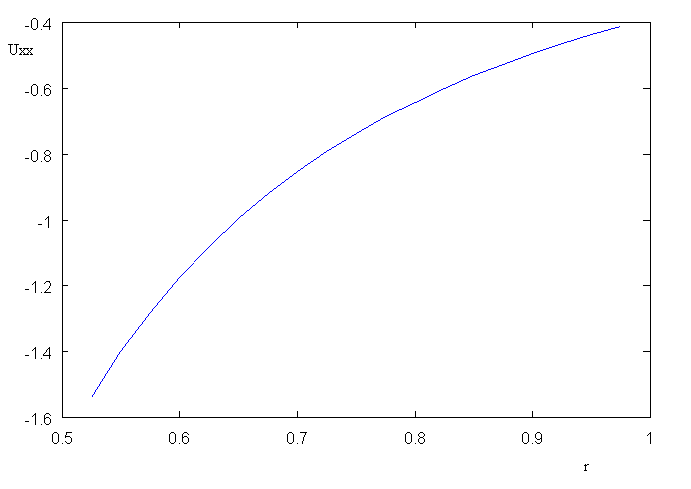
\includegraphics[scale=0.2]{./img/uxx.png}
	\end{center}
\end{figure}
\begin{center}
\par Figura 1: Derivada segunda de u respecto a r para $t=10$.
\end{center}

Del gráfico se puede apreciar que la derivada segunda es negativa, por lo que el error es positivo. Es decir, 
se subestima el valor de la deformación. Por otro lado, es evidente que $2$ es una cota apropiada para el 
módulo de dicha derivada. Por lo que:

\[
e_{trap} = \frac{\Delta r^2}{12}
\]
En otras palabras, el error de aproximar la integral por el método del trapecio es equivalente a un doceavo 
del paso en el radio usado, para $t=10$. Nótese que este error contempla únicamente el error por utilizar 
dicho método y no el error por aproximar $u(r,t)$ utilizando $v(r,t)$.

\section{Resultados}

\subsection{Temperaturas para distintos radios}

El siguiente gráfico muestra temperaturas para distintos radios en función del tiempo. Se utilizó $\Delta r = 0.025$ 
y $\Delta t = 0.0005$. Se puede apreciar que la temperatura incrementa en el tiempo, y además es menor 
para menores valores del radio.

\begin{figure}[H]
	\begin{center}
	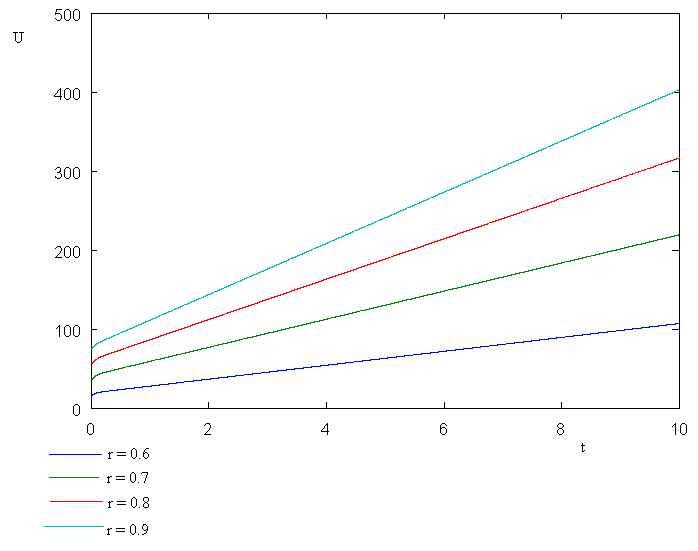
\includegraphics[scale=0.33]{./img/r.png}
	\end{center}
\end{figure}
\begin{center}
\par Figura 2: Temperatura en función del tiempo para distintos radios.
\end{center}

En el siguiente gráfico se demuestra la temperatura en función del radio y el tiempo, utilizando $\Delta r = 0.1$ y 
$\Delta t = 0.001$. Las conclusiones extraídas del mismo son equivalentes a las del gráfico anterior.

\begin{figure}[H]
	\begin{center}
	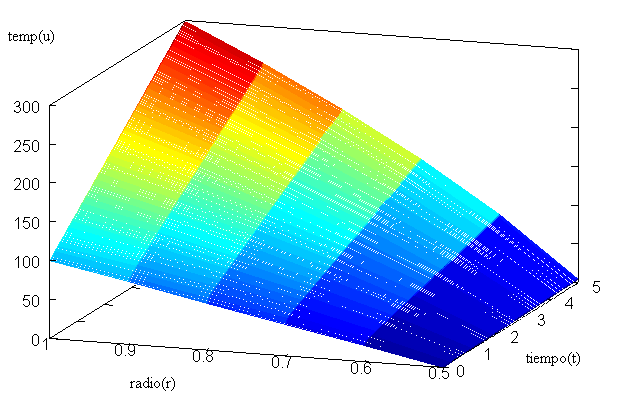
\includegraphics[scale=0.4]{./img/mesh.png}
	\end{center}
\end{figure}
\begin{center}
\par Figura 3: Temperatura en función del tiempo y el radio.
\end{center}

\subsection{Deformación}

La figura 4 demuestra la deformación en función del tiempo. Se utilizó nuevamente $\Delta r = 0.025$ 
y $\Delta t = 0.0005$. Nótese que la deformación incrementa con el tiempo, lo cual es esperable debido a 
que la temperatura también lo hace. Por otro lado, se puede apreciar que el incremento es lineal.

\begin{figure}[H]
	\begin{center}
	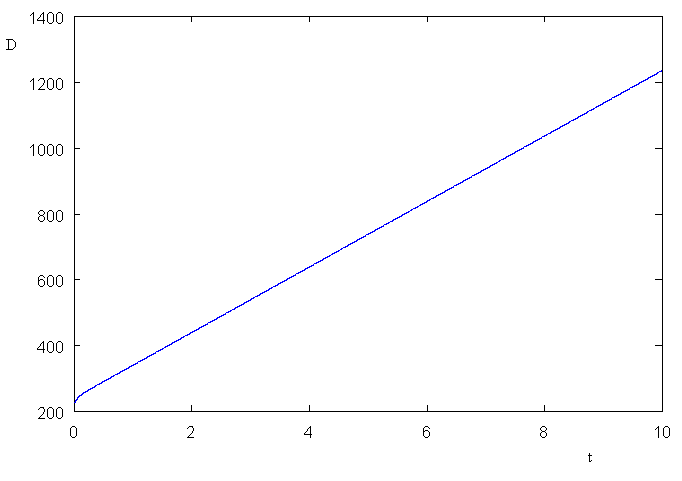
\includegraphics[scale=0.4]{./img/deformacion.png}
	\end{center}
\end{figure}
\begin{center}
\par Figura 4: Deformación en función del tiempo.
\end{center}

\subsection{Isotermas}

En la figura dos se pueden apreciar las isotermas de la solución. Estas serían las curvas resultantes de 
la intersección de los planos para distintas temperaturas con la solución. El siguiente gráfico (figura 5) muestra 
las curvas para distintas temperaturas, llevadas todas a un mismo plano para poder representarlas en dos dimensiones.

\begin{figure}[H]
	\begin{center}
	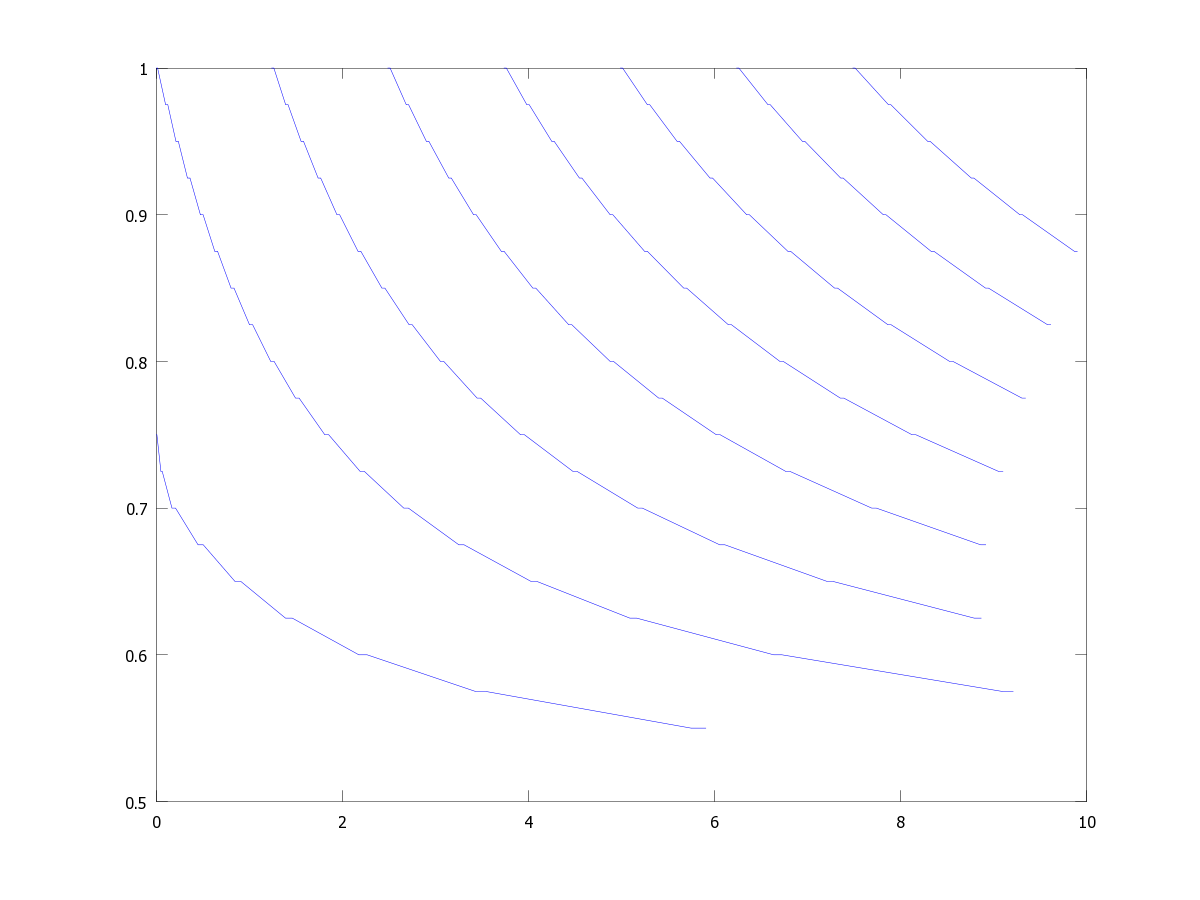
\includegraphics[scale=0.2]{./img/isotemps.png}
	\end{center}
\end{figure}
\begin{center}
\par Figura 5: Isotermas para u = 50,100,150,200,250,300,350,400, de izquierda a derecha.
\end{center}

\subsection{Utilización de pasos no estables}

Los siguientes gráficos muestran la temperatura en función del radio para tiempos sucesivos. Se utilizó un 
paso de $\Delta r = 0.1$ y \Delta t= 0.1$. Nótese que para estos valores $p=4$, lo cual es inestable según \eqref{p}. 

\begin{figure}[H]
	\begin{center}
	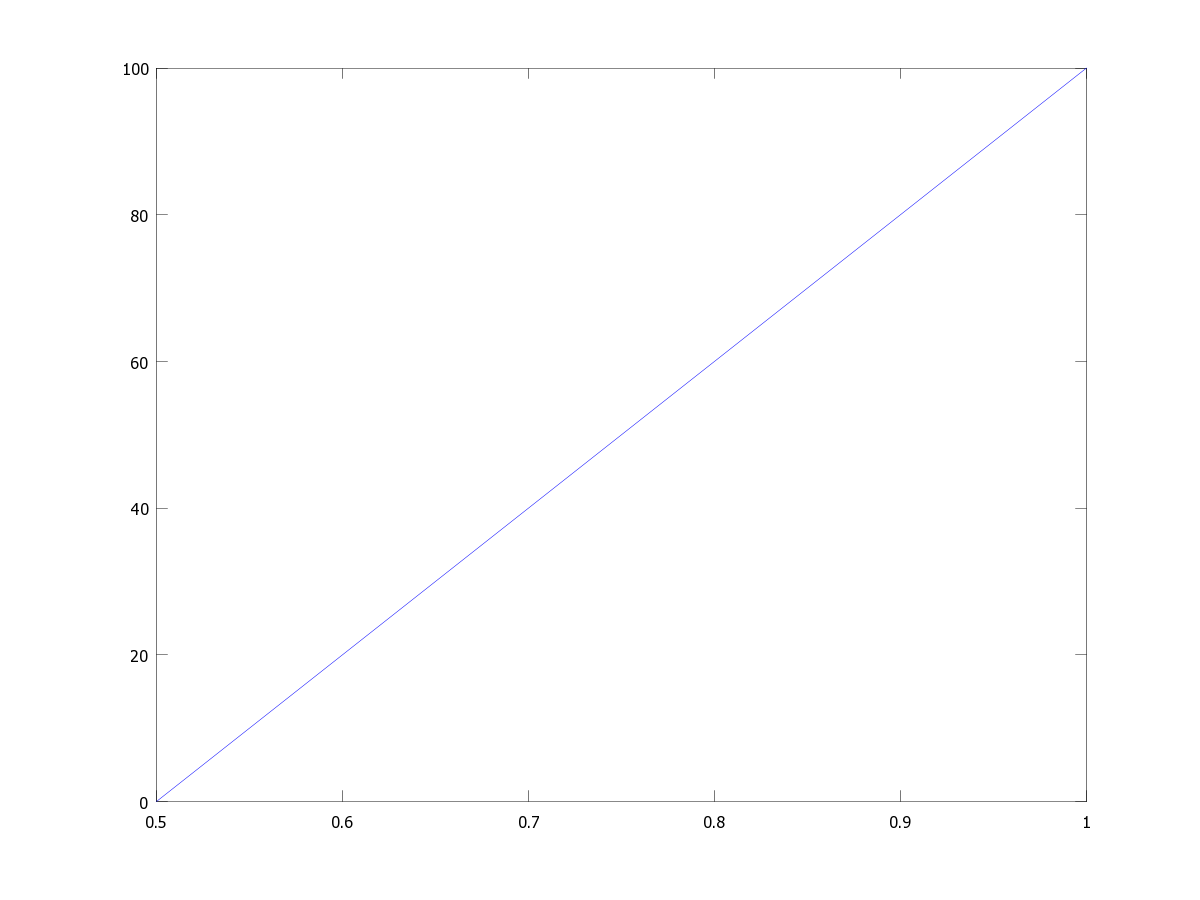
\includegraphics[scale=0.2]{./img/div1.png}
	\end{center}
\end{figure}
\begin{center}
\par Figura 6: Temperatura en función del radio, para $t=0.0$.
\end{center}

\begin{figure}[H]
	\begin{center}
	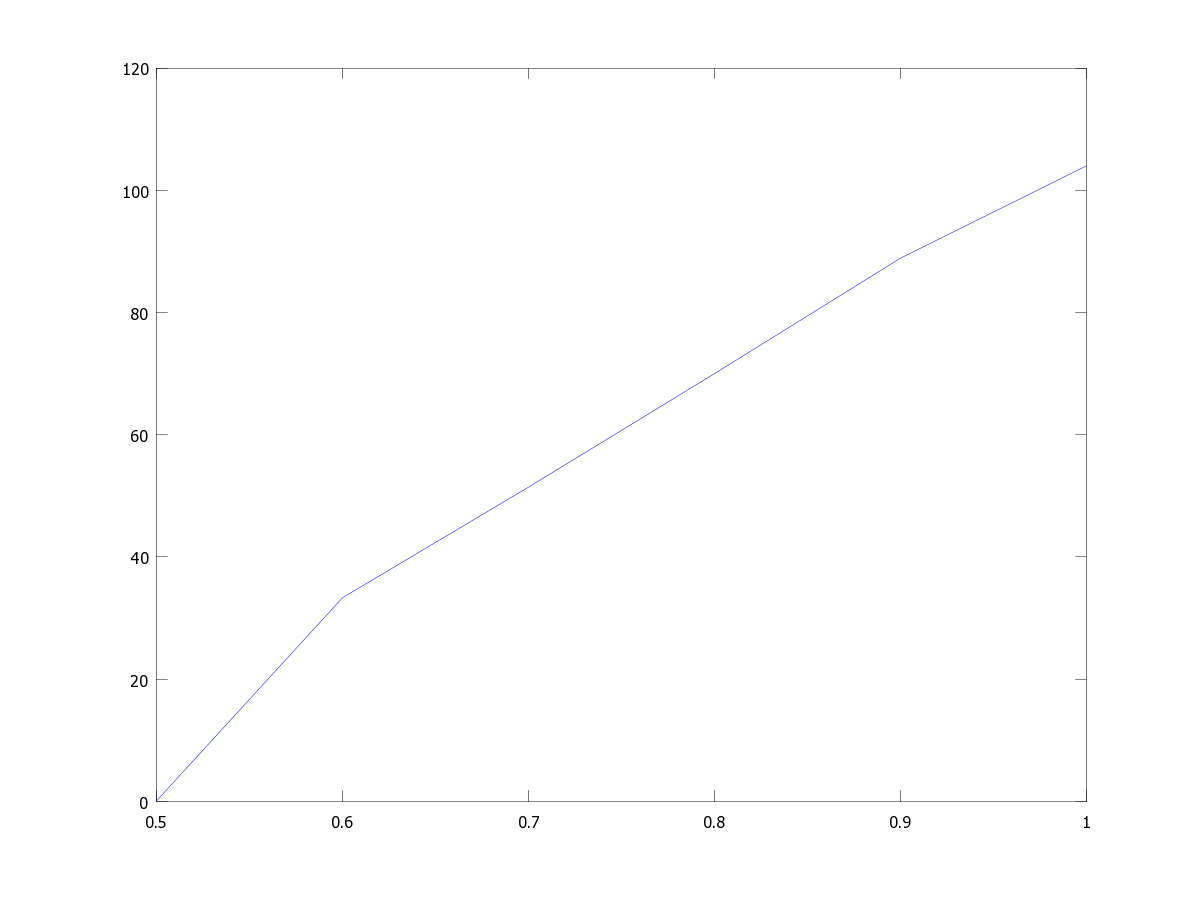
\includegraphics[scale=0.2]{./img/div2.png}
	\end{center}
\end{figure}
\begin{center}
\par Figura 7: Temperatura en función del radio, para $t=0.1$.
\end{center}

\begin{figure}[H]
	\begin{center}
	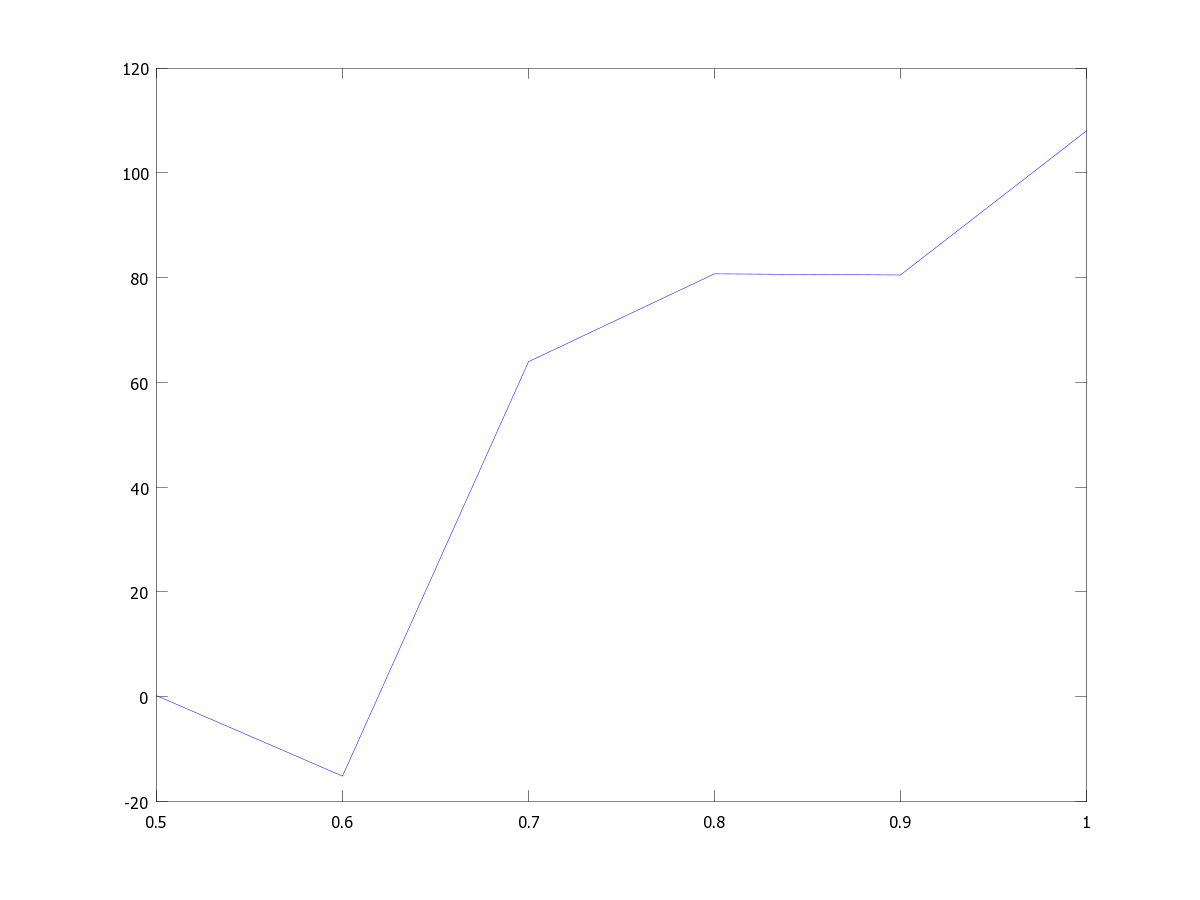
\includegraphics[scale=0.2]{./img/div3.png}
	\end{center}
\end{figure}
\begin{center}
\par Figura 8: Temperatura en función del radio, para $t=0.2$.
\end{center}

\begin{figure}[H]
	\begin{center}
	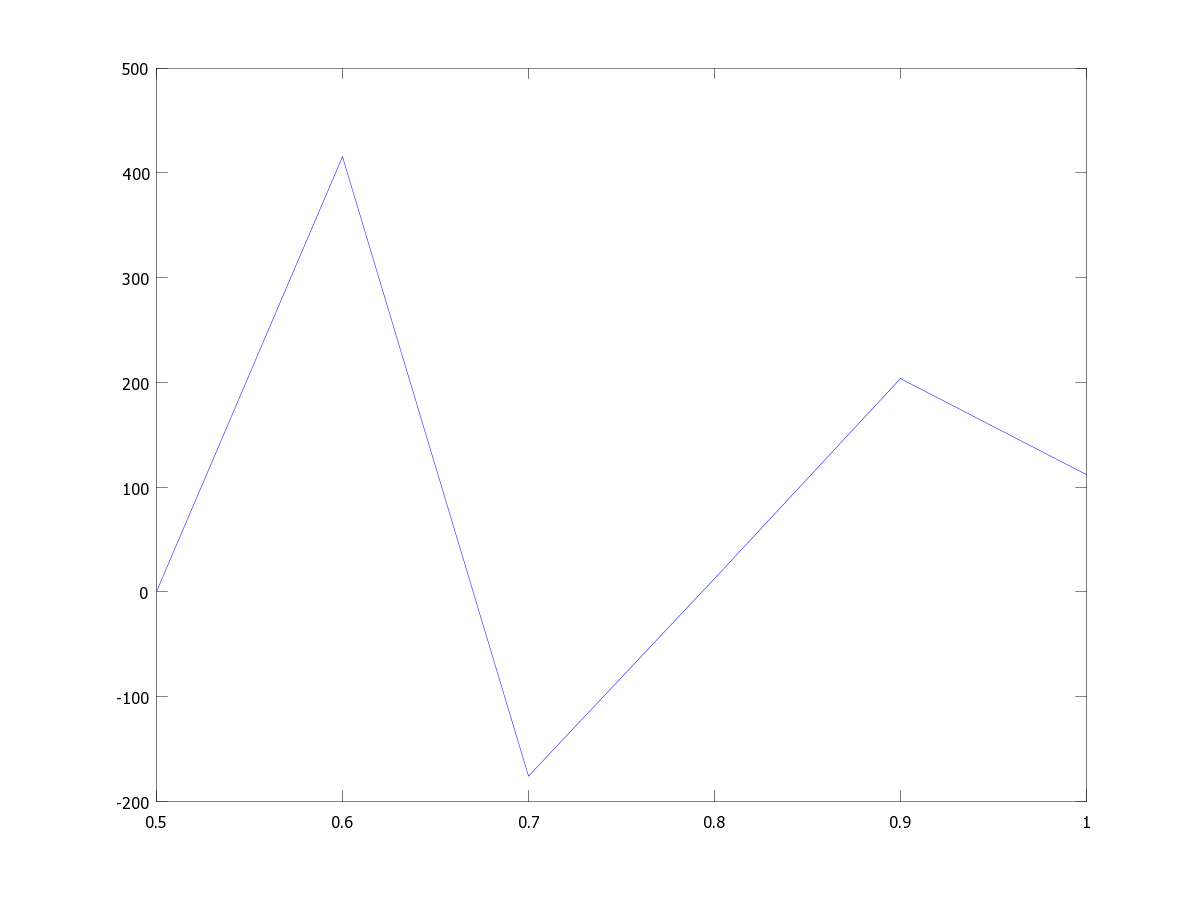
\includegraphics[scale=0.2]{./img/div4.png}
	\end{center}
\end{figure}
\begin{center}
\par Figura 9: Temperatura en función del radio, para $t=0.3$.
\end{center}

\begin{figure}[H]
	\begin{center}
	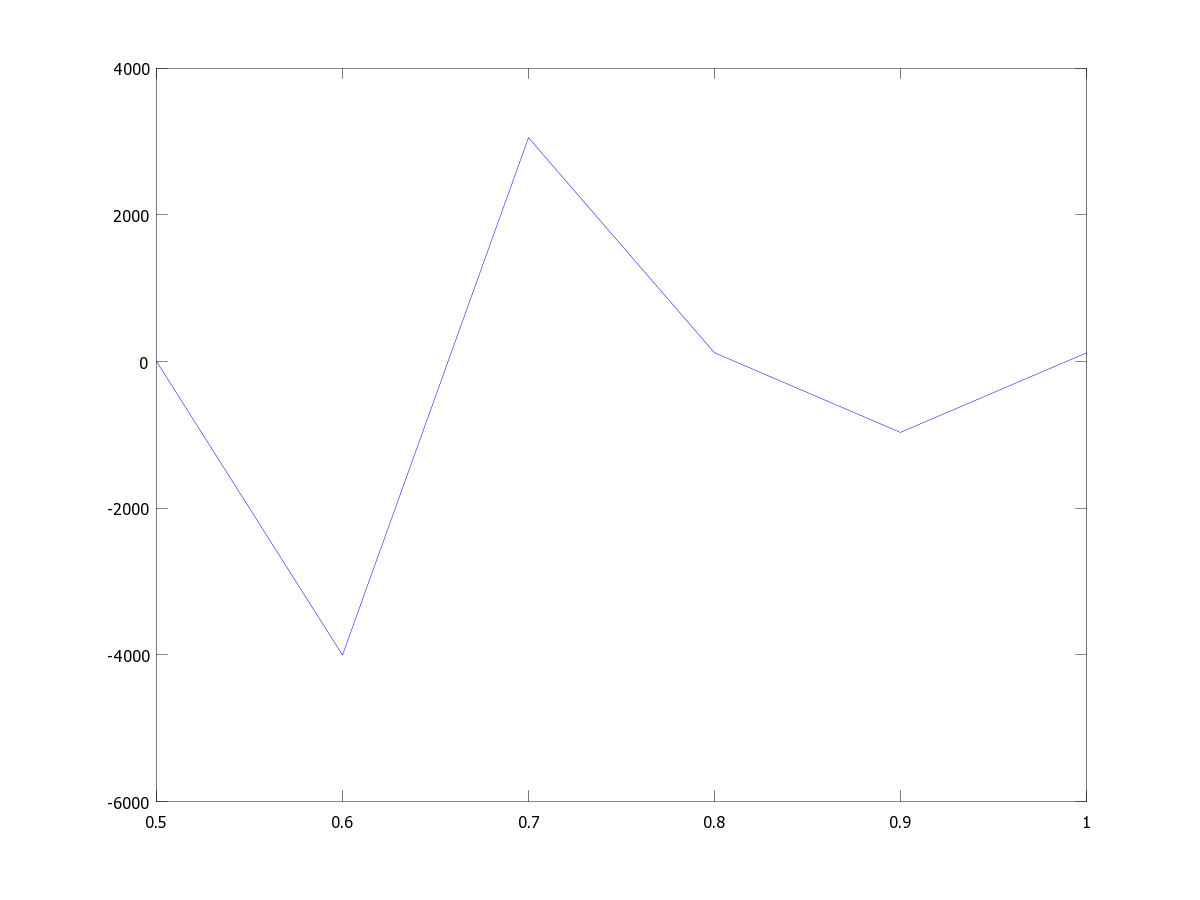
\includegraphics[scale=0.2]{./img/div5.png}
	\end{center}
\end{figure}
\begin{center}
\par Figura 10: Temperatura en función del radio, para $t=0.4$.
\end{center}

\begin{figure}[H]
	\begin{center}
	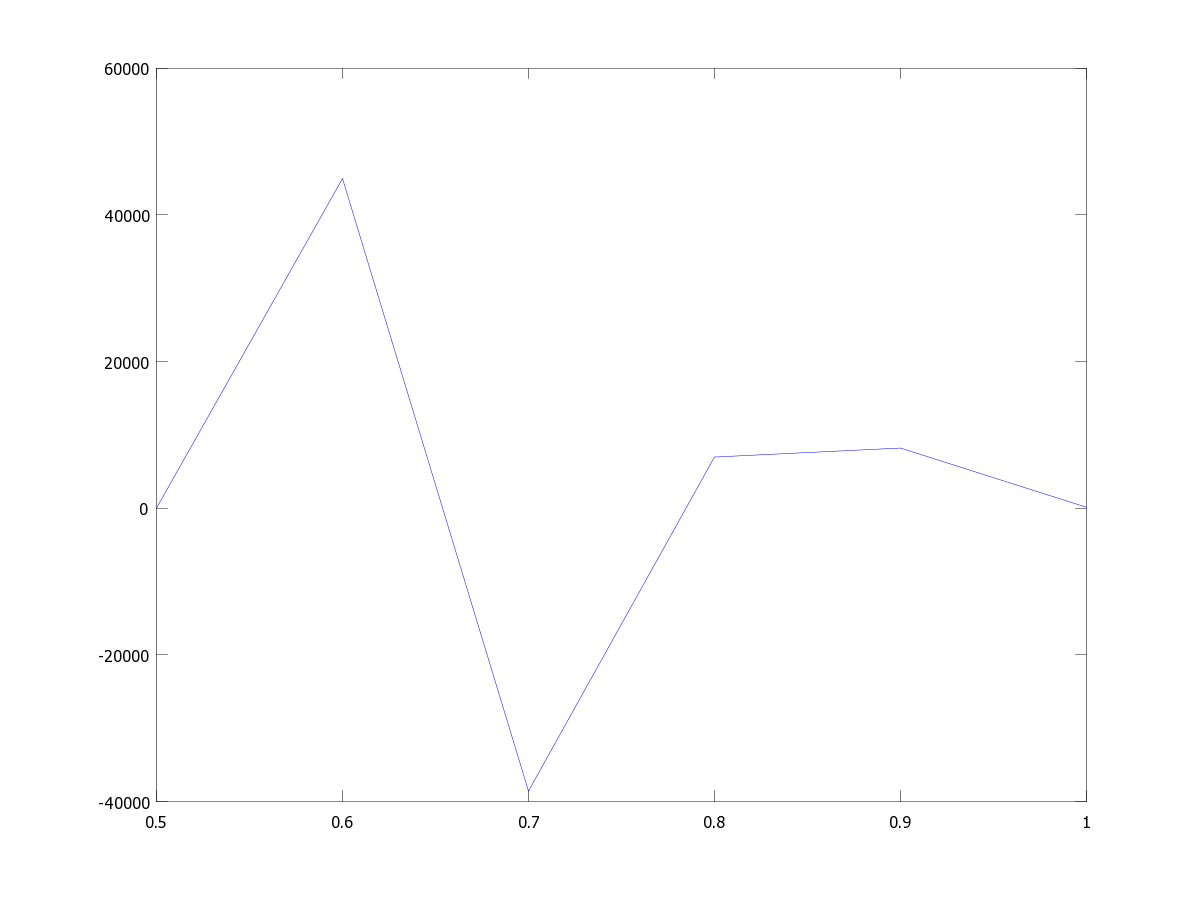
\includegraphics[scale=0.2]{./img/div6.png}
	\end{center}
\end{figure}
\begin{center}
\par Figura 11: Temperatura en función del radio, para $t=0.5$.
\end{center}

\par De los gráficos se puede apreciar cómo rápidamente la temperatura comienza a diverger. Esto se debe 
al uso de pasos inestables, lo cual demuestra la importancia de garantizar la estabilidad de la aproximaciones 
utilizando ecuaciones en diferencias.

\begin{thebibliography}{1}


\bibitem{lamport1}
\newblock {\em{  Regla del trapecio - http://en.wikipedia.org/wiki/Trapezoidal\_rule}}
\bibitem{lamport1}
\newblock {\em{ Ecuaciones en diferencias - http://en.wikipedia.org/wiki/Finite\_difference}}

\end{thebibliography}




\clearpage

\onecolumn

\section*{Anexo A: Código Octave}

\VerbatimInput{../src/main.m}

\section*{Anexo B: Deducción ecuación en diferencias}

\begin{equation}
\frac{\partial^2 u}{\partial r^2}+\frac{1}{r}\frac{\partial u}{\partial r}=\frac{1}{4K}\frac{\partial u}{\partial t}
\end{equation}

\[ \frac{v(n+1,t) - 2v(n,t) + v(n-1,t)}{\Delta r^2} + \frac{v(n+1,t) - v(n,t)}{r\Delta r} = \frac{1}{4K}\frac{v(n,t+1) - v(n,t)}{\Delta t} \]

Sea $p=\frac{\Delta t4K}{\Delta r^2}$ y $q=\frac{\Delta r}{r}$.
\[ p\left( v(n+1,t) - 2v(n,t) + v(n-1,t) + q\left( v(n+1,t) - v(n,t) \right) + v(n,t) = v(n, t+1) \]

Lo cual se reduce a:

\begin{equation}
p(1+q)v(n+1,t) + (1-p(2+q))v(n,t) + pv(n-1,t) = v(n,t+1)
\end{equation}

\section*{Anexo C: Derivada}

\[
2(4p^2+4p^2q+p^2q^2) cos(\omega)sen(\omega) - 2sen(\omega)(2p+pq)(1-p(2+q))+2p^2q^2cos(\omega)sen(\omega) = 0
\]


